\documentclass[12pt, a4paper]{scrreprt}

\usepackage[tight]{shorttoc}
\usepackage{pgfplots, amssymb, todonotes, pdfpages, mystyle, tabularx, booktabs, tcolorbox, mathtools}
\usetikzlibrary{angles, arrows}
\pgfplotsset{compat=1.16}
\pgfplotsset{
  width=7cm,
  grid = major,
  axis lines = center,
}
%\newcommand{\im}{\textcolor{red}{i}
%\newcommand{\laplace}{\textcolor{red}{LAPLACE}

% \setlength{\extrarowheight}{12pt}
\begin{document}

\newgeometry{margin=1.5cm}
\begin{titlepage}

  \includesvg[width=0.25\textwidth]{Grafiken/LogoHS_Esslingen}\\ \vspace{3cm}
  
  \begin{center}
    {\usekomafont{disposition}
      \Huge Formelsammlung Mathematik 3}
    \vspace{0.5cm}
    
    \begin{Large}
      Tim Hilt\\
      \vspace{0.4cm}
      \today\\
    \end{Large}
    
  \end{center}
\end{titlepage}
\restoregeometry

%%% Local Variables:
%%% mode: latex
%%% TeX-master: "Mathe3Formelsammlung"
%%% End:

\shorttoc{Kurzes Inhaltsverzeichnis}{1}
\tableofcontents
\clearpage

\chapter{Grundlagen und Wiederholung}

\section{Allgemeine trigonometrische Umformungen; Additionstheoreme und Doppelwinkelformeln}

\bgroup
\def\arraystretch{1.5}
\begin{center}
  \begin{tabularx}{.7\textwidth}{rXl}
    \(\tan x\) & \(=\) & \(\frac{\sin x}{\cos x}\)\\
    \(\sin ^2 x + \cos ^2 x\) & \(=\) & \(1\)\\[1em]
    \(\sin ( x \pm y )\) & \(=\) & \(\sin x \cos y \pm \cos x \sin y\)\\
    \(\cos ( x \pm y )\) & \(=\) & \(\cos x \cos y \mp \sin x \sin y\)\\
    \(\tan ( x \pm y )\) & \(=\) & \(\frac{\tan x \pm \tan y}{1 \mp \tan x \tan y} = \frac{\sin ( x \pm y )}{\cos ( x \pm y )}\)\\[1em]
    \(\sin (2x)\) & \(=\) &  \(2 \sin x \cos x\)\\
    \(\cos (2x)\) & \(=\) & \(\cos ^2 x - \sin ^2 x = 1 - 2 \sin ^2 x = 2 \cos ^2 x - 1\)\\
    \(\tan (2x)\) & \(=\) & \(\frac{2 \tan x}{1 - \tan ^2 x}\)
  \end{tabularx}
\end{center}
\egroup

\section{Komplexe Zahlen}

\subsection{Darstellungsformen komplexer Zahlen}

\begin{center}
  \begin{tabularx}{\textwidth}{XX}
    \toprule
    Kartesische Form: & \(z = x + \im y\)\\
    Polarform; Polarkoordinaten: & \(z = r \cos \varphi + \im r \sin \varphi\)\\
    Exponentialform: & \(r e^{\im \varphi}\)\\
    \bottomrule
  \end{tabularx}

  \begin{tikzpicture}
    \begin{axis}[
      ymin = -0.5,
      xmin = -0.5,
      xmax = 2,
      ymax = 2,
      xtick distance = 1,
      ytick distance = 1,
      grid = none,
      xlabel = \(\operatorname{Re}\),
      ylabel = \(\operatorname{Im}\),
      extra x ticks = {1.6},
      extra y ticks = {1.3},
      extra x tick label = {\(x\)},
      extra y tick label = {\(y\)},
      width = \textwidth,
      ]
      \draw [->, >=stealth, very thick, myred] (axis cs:0,0) -- (axis cs:1.6, 1.3) node [sloped, above, midway] {\(r\)};
      \draw [dotted] (axis cs:0,1.3) -- (axis cs:1.6,1.3);
      \draw [dotted] (axis cs:1.6,0) -- (axis cs:1.6,1.3);
      \path (axis cs:1.6,1.3) node [myred, above] {\(z\)};
      \filldraw [fill = myred!20, draw = myred] (axis cs:0,0) -- (axis cs:0.5,0) arc [start angle=0, end angle=36.5, radius=2.7cm] -- cycle;
      \path (axis cs:0.3,0.11) node [myred] {\(\varphi\)};
    \end{axis}
  \end{tikzpicture}
\end{center}

\subsection{Umrechnung verschiedener Darstellungsformen ineinander}

\begin{mybox}
  \(
  \begin{aligned}
    z &= r \cos \varphi + \im r \sin \varphi = r e^{\im \varphi}\\
    r &= |z| = \sqrt{x^2 + y^2}
  \end{aligned}
  \)
\end{mybox}

\begin{mathframed}
  \arg (z) = \varphi =
  \begin{cases}
    \arctan \left(\frac{y}{x}\right) & \text{für } x>0, y \text{ bel.}\\
    \arctan \left(\frac{y}{x}\right) + \pi & \text{für } x<0, y \geq 0\\
    \arctan \left(\frac{y}{x}\right) + \pi & \text{für } x<0, y<0\\
    \frac{\pi}{2} & \text{für } x = 0, y > 0\\
    - \frac{\pi}{2} & \text{für } x = 0,y < 0
  \end{cases}
\end{mathframed}

\subsection{Darstellung Sinus und Kosinus als komplexe Zahlen}

Zudem können Kosinus und Sinus auch dargestellt werden durch:

\begin{mathframed}
  \cos \varphi = \frac{e^{\im \varphi} + e^{- \im \varphi}}{2} \qquad
  \sin \varphi = \frac{e^{\im \varphi} - e^{- \im \varphi}}{2 \im}
\end{mathframed}

\section{Sinus Kardinalis}

\begin{minipage}{.5\linewidth}
Der Sinus Kardinals \(\operatorname{si}(x)\) ist definiert als

\[
  \operatorname{si}(x)=
  \begin{cases}
    \frac{\sin(x)}{x} & x \in \mathbb{R} \backslash 0\\
    1 & x = 0
  \end{cases}
\]
\end{minipage}%
\begin{minipage}{.5\linewidth}
  \begin{center}
    \begin{tikzpicture}
      \begin{axis}[
          xmin = -4*pi,
          xmax = 4*pi,
          samples = 200,
          ]
        \addplot[myred,very thick,domain=-4*pi:4*pi]{sin(deg(x))/x};
      \end{axis}
    \end{tikzpicture}
  \end{center}
\end{minipage}

\begin{minipage}{.5\linewidth}
  Eine spezielle Form ist die \(\operatorname{sinc}(x)\)-Funktion. Sie ist definiert als:
  \[
    \operatorname{sinc}(x)=
    \begin{cases}
      \frac{\sin(\pi x)}{\pi x} & x \in\mathbb{R} \backslash 0\\
      1 & x = 0
    \end{cases}
  \]
\end{minipage}%
\begin{minipage}{.5\linewidth}
  \begin{center}
    \begin{tikzpicture}
      \begin{axis}[
          xmin = -4*pi,
          xmax = 4*pi,
          samples = 200,
          ]
        \addplot[myred,very thick,domain=-4*pi:4*pi]{(sin(deg(pi*x)))/(pi*x)};
      \end{axis}
    \end{tikzpicture}
  \end{center}
\end{minipage}

\part{Transformationen und Verallgemeinerte Funktionen}

\chapter{Verallgemeinerte Funktionen}

\section{Heaviside-Funktion}
\begin{minipage}{.5\textwidth}
  Die Heaviside-Funktion oder Einheitssprungfunktion ist definiert durch:
  \[
    \sigma (t) =
    \begin{cases}
      0 & t \in (-\infty, 0]\\
    1 & t \in (0, \infty)
  \end{cases}
\]
\end{minipage}\hfill%
\begin{minipage}{.5\textwidth}
  \centering
  \begin{tikzpicture}
    \begin{axis}[xmin = -5,
        xmax = 5,
        ymin = -1,
        ymax = 2,
        legend entries = {\(\sigma(t)\)},
        ]
      \addplot[domain=-5:0, myred, very thick] {0};
      \addplot[domain=0:5, myred, very thick] {1};
    \end{axis}
  \end{tikzpicture}
\end{minipage}

\begin{minipage}{.5\textwidth}
  Wird eine Funktion mit der Heaviside-Funktion multipliziert, so werden Teile der Funktion ausgeblendet.
\end{minipage}\hfill%
\begin{minipage}{.5\textwidth}
  \centering
  \begin{tikzpicture}
    \begin{axis}[]
      \addplot [domain=0:5, myred, very thick] {x^2+5};
      \addplot [domain=-5:0, blue, very thick] {0};
    \end{axis}
  \end{tikzpicture}
\end{minipage}

\begin{minipage}{.5\textwidth}
  Mithilfe der Heaviside-Funktion können Rechteckimpulse erstellt werden.

  \begin{framed}
    \[
      r(t) = \sigma (t-t_0) - \sigma (t-t_1)
    \]
  \end{framed}
\end{minipage}\hfill%
\begin{minipage}{.5\textwidth}
  \centering
  \begin{tikzpicture}
    \begin{axis}[
        ymax=1.5,
        xmin = -1,
        xmax = 3,
        xtick = {1,2},
        xticklabels={
          \(t_0\),
          \(t_1\),
        },
        ]
      % Wenn mans umständlich machen will:
      %
      % \addplot [domain = -5:1, myred, very thick] {0};
      % \addplot [domain = 1:2, myred, very thick] {1};
      % \addplot [domain = 2:5, myred, very thick] {0};
      % \draw [very thick, myred] (axis cs:1,0) -- (axis cs:1,1);
      % \draw [very thick, myred] (axis cs:2,0) -- (axis cs:2,1);
      %
      % Wenn mans klug machen will:
      \addplot [myred, very thick] coordinates {
        (-5, 0)
        (1, 0)
        (1, 1)
        (2, 1)
        (2, 0)
        (5, 0)
      };
    \end{axis}
  \end{tikzpicture}
\end{minipage}

\section{Dirac-Distribution}
\begin{minipage}{.5\textwidth}
  Die Dirac-Distribution ist definiert durch:
  \[
    \delta(x)=
    \begin{cases}
      0 & t \in \mathbb{R} \backslash 0\\
      1 & t = 0\\
    \end{cases}
  \]
\end{minipage}\hfill%
\begin{minipage}{.5\textwidth}
  \centering
  \begin{tikzpicture}
    \begin{axis}[
        xmin = -5,
        xmax = 5,
        ymin = -1,
        ymax = 2,
        legend entries = {\(\delta(t)\)},
        ]
      \addplot[myred, very thick] {0};
      \draw[->, very thick, myred, >=stealth] (axis cs:0,0) -- (axis cs:0,1);
    \end{axis}
  \end{tikzpicture}
\end{minipage}

Genauer wird die Dirac-Distribution durch eine Folge von Rechteckimpulsen hergeleitet, die den konstanten Flächeninhalt \(1\) besitzen, deren Breite dabei jedoch gegen \(0\) strebt, deren Höhe dafür aber gegen \(\infty\).

\begin{minipage}{.5\textwidth}
  Wird eine Funktion mit der Dirac-Distribution an einem Punkt \(t\) multipliziert, so wird die \textbf{gesamte Funktion, bis auf den Funktionswert an der Stelle \(t\) ausgeblendet!}
\end{minipage}\hfill%
\begin{minipage}{.5\textwidth}
  \centering
  \begin{tikzpicture}
    \begin{axis}[
        xmin = 0,
        xmax = 5,
        ymin = -1,
        ymax = 5,
        samples = 50,
        ]
      \addplot [gray] {(x-2)^2+2};
      \draw [->, >=stealth, myred, very thick] (axis cs:3,0) -- (axis cs:3,3);
    \end{axis}
  \end{tikzpicture}
  {\footnotesize \((t-2)^2+2 \cdot \delta(t-3)\)}
\end{minipage}

\section{Verallgemeinerte Ableitung}

Leitet man die Heaviside-Funktion ab entsteht die Dirac-Distribution.

\begin{framed}
  \[
    \dot{\sigma} (t) = \delta (t)
  \]
  \mybfcol{Beim Ableiten ist insbesondere auf die innere Ableitung zu achten!}
\end{framed}

\subsection{Grafisches Ableiten verallgemeinerter Funktionen}

\begin{minipage}{.45\textwidth}
  Wird eine Funktion mit Unstetigkeitsstellen abgeleitet, so wird an der Sprungstelle ein Dirac-Impuls in Höhe und Richtung des Sprungs eingezeichnet. Dieser Impuls ist von der \(x\)-Achse aus zu zeichnen.
\end{minipage}\hfill%
\begin{minipage}{.45\textwidth}
  \begin{tikzpicture}
    \begin{axis}[
        axis lines = center,
        ymin = -1.5,
        ymax = 1.5,
        ytick distance = 0.5,
        xtick distance = 1,
        xlabel = \(t\),
        ylabel = \(y\),
        legend pos = outer north east,
        ]
      \addlegendentry{\(f(t)\)}
      \addlegendentry{\(\dot{f} (t)\)}
      \addplot [myred, very thick] coordinates {
        (-2, -0.5)
        (0, -0.5)
      };
      \addplot [mygreen, very thick] coordinates {
        (-2, 0)
        (0, 0)
        (1, 2)
      };
      \addplot [domain = 0:1, myred, very thick] {x^2};
      \addplot [myred, very thick] coordinates {
        (1, 0.5)
        (2, 0.5)
      };
      \addplot[mygreen, very thick] coordinates {
        (1, 0)
        (2, 0)
      };
      \draw [->, >=stealth, color= mygreen, very thick] (axis cs:0,0) -- (axis cs:0,0.5);
      \draw [->, >=stealth, color= mygreen, very thick] (axis cs:1,0) -- (axis cs:1,-0.5);
    \end{axis}
  \end{tikzpicture}
\end{minipage}

Jedoch kann die Dirac-Distribution mit unserem Wissensstand nicht weiter abgeleitet werden.

\section{Faltung}

\glqq{}A convolution is an integral that expresses the amount of overlap of one function \(g\) as it is shifted over another function \(f\).\grqq{} (\href{http://mathworld.wolfram.com/Convolution.html}{\texttt{http://mathworld.wolfram.com/Convolution.html}})

Die Faltung ist definiert durch:

\begin{mathframed}
  h(t) = f(t) \star g(t) = \int_{-\infty}^{\infty}f(\tau) \cdot g(t-\tau) d \tau
\end{mathframed}

Dadurch entsteht eine neue Funktion \(h(t)\). \(\tau\) ist eine Dummy-Variable! Beim Integrieren verschwindet sie und bildet die Funktion wieder auf~ \(t\) ab.


\section{Faltung mit \(\sigma (t)\)}

Wird eine Funktion mit \(\sigma (t)\) gefaltet, so ergibt sich für das Faltungsintegral:

\[
  (t) \star \sigma (t) = \int_{-\infty}^{\infty} f(\tau) \cdot \sigma(t - \tau) d\tau = \int_{-\infty}^t f(\tau) d\tau
\]

\section{Faltung mit \(\delta(t)\)}

Wird eine Funktion \(f(t)\) mit der Dirac-Distribution \(\delta (t)\) gefaltet, so ergibt sich:

\[
  f(t) \star \delta(t) = \int_{-\infty}^{\infty} f(\tau) \cdot \delta(t - \tau) d\tau = f(t)
\]

Dies haben wir den Ausblendeigenschaften der Dirac-Distribution zu verdanken.

\section{Einseitige Faltung}

Sind beide Funktionen \(f(t)\)~und \(g(t) = 0\)~für \(x \leq 0\), so ergibt sich das Faltungsintegral:

\[
  f(t) \star g(t) = \int_0^t f(\tau) \cdot g(t - \tau) d\tau
\]

\chapter{Fourier-Transformation}

Mithilfe der Fouriertransformation werden Funktionen aus dem Zeitbereich in den Frequenzbereich übersetzt:

\begin{mathframed}
  s(t)~\laplace~S(f) = \int_{-\infty}^{\infty} s(t) e^{- \im 2\pi ft} dt
\end{mathframed}

\section{Real- und Imaginärteil direkt berechnen}

In der Regel ist das Ergebnis einer Fouriertransformation eine komplexwertige Funktion. Natürlich lässt sich diese stets in Real- und Imaginärteil aufspalten --- die Anteile lassen sich aber auch direkt berechnen:

\begin{mathframed}
  \operatorname{Re} (z) &= \int_{- \infty}^{\infty} s(t)\ \cos (2\pi f t)\ dt\\[1em]
  \operatorname{Im} (z) &= -\int_{- \infty}^{\infty} s(t)\ \sin (2\pi f t)\ dt
\end{mathframed}

\clearpage

\section{Fourier-Transformation von geraden- und ungeraden Funktionen}

Ist die zu transformierende Funktion \mybfcol{gerade}, so ist die Transformierte \mybfcol{rein reell und ebenfalls gerade}, aufgrund der Symmetrieeigenschaften des Kosinus. Zudem muss nicht mehr von \(- \infty\) bis \(\infty\) integriert werden. Es genügt das Integral von \(0\) bis \(\infty\) mit \(2\) zu multiplizieren. Ihre Berechnung reduziert sich dabei auf:

\begin{mathframed}
  S(f) = \operatorname{Re}(f) = 2 \int_{0}^{\infty} s(t)\ \cos (2\pi f t) dt
\end{mathframed}

Das selbe Prinzip lässt sich auf die Berechnung \mybfcol{ungerader} Funktionen anwenden. Hier ist die Transformierte \mybfcol{rein imaginär und ungerade}:

\begin{mathframed}
  S(f) = \im \operatorname{Im}(f) = -2\im \int_{0}^{\infty}s(t)\ \sin (2\pi f t) dt
\end{mathframed}

\section{Darstellung mit Amplituden- und Phasenwinkel}

Fourierreihen lassen sich auch in Exponentialform darstellen:

\begin{mathframed}
  S(f) = |S(f)| e^{\im\varphi (f)}
\end{mathframed}

Dabei ist
\begin{itemize}
\item Die Amplitude \(|S(f)| = \sqrt{\operatorname{Re}(f)^2 + \operatorname{Im}(f)^2}\) eine \mybfcol{gerade, reelle} Funktion
\item Die Phase \(\varphi(f) = \arg (S(f)) = \arg (\operatorname{Re}(f) + \im\operatorname{Im}(f))\) eine \mybfcol{ungerade, reelle} Funktion.
\end{itemize}

Diese Darstellung findet insbesondere in der Elektrotechnik ihre Anwendung (Bode-Diagramm).

\section{Inverse Fourier-Transformation}

Um aus einer fouriertransormierten Funktion \(S(f)\) die Zeitfunktion \(s(t)\) zu erhalten muss \(S(f)\) \textbf{rücktransformiert} werden:


\begin{mathframed}
  S(f)~\Laplace~s(t) = \int_{-\infty}^{\infty} S(f) e^{\im 2 \pi f} df
\end{mathframed}

\clearpage

\chapter{Laplacetransformation}

  Die Berechnung der Laplace-Transformation ist definiert durch:
  
\begin{mathbox}
    f(t)~\laplace~F(s) = \int_0^{\infty}f(t) \cdot e^{-st} dt
\end{mathbox}
\chapter{z-Transformation}

\part{Statistik und Wahrscheinlichkeitsrechnung}

\chapter{Beschreibende Statistik}

\chapter{Kombinatorik und Wahrscheinlichkeitsrechnung}

\section{Kombinatorik}

\subsection{Permutation}

\begin{tabular}{lc}
  \toprule
  Permutation ohne Wiederholung: & \(n!\)\\
  \midrule
  Permutation mit Wiederholung: & \(\displaystyle{\frac{n!}{k_1! \cdot k_2! \cdot \ldots \cdot k_s!}}\)\\
  \bottomrule
\end{tabular}

\section{Kombination und Variation}

Kombinationen werden verwendet, wenn \textbf{nur einige} der Elemente in einer Menge angeordnet werden sollen. Permutationen hingegen ordnen \textbf{alle} Elemente an.

\begin{figure}[H]
  \centering
  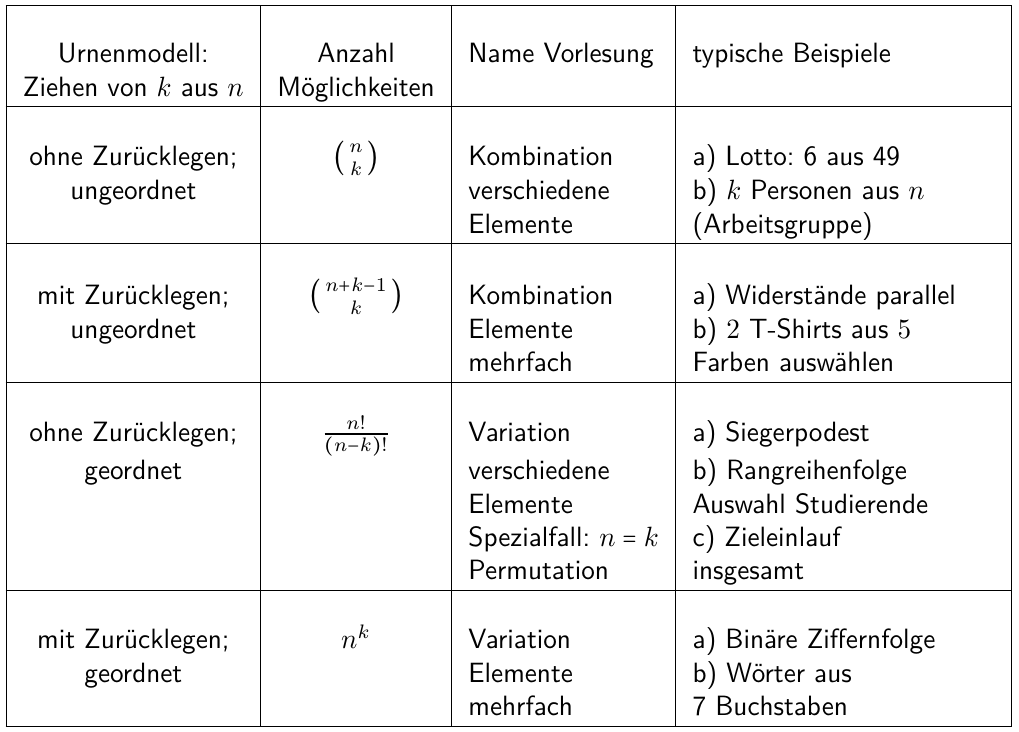
\includegraphics[width=\textwidth]{Grafiken/Kombinatorik}
\end{figure}

\section{Wahrscheinlichkeitsrechnung}

\subsection{Wahrscheinlichkeitsverteilungen}

\begin{figure}[H]
  \subsubsection{Allgemeine Form}
  \textbf{Dichtefunktion:}

  Funktion, bei der auf der \(x\)-Achse alle Elemente mit der auf der \(y\)-Achse aufgetragenen Wahrscheinlichkeit gezeichnet sind. Es ergibt sich ein Säulendiagramm.

  \textbf{Verteilungsfunktion:}
  \[F(x) = P(X \leq x) = \sum_k^x(k \cdot P(X=k))\]
  \textbf{Erwartungswert:}
  \[E(X) = \mu = \sum_k k \cdot P(X=k)\]
  \textbf{Varianz}
  \[\operatorname{Var}(X) = \sigma^2 = \sum_k {(k^2 \cdot P(X=k) )} - \mu^2\]
\end{figure}

\begin{figure}[H]
  \subsubsection{Hypergeometrische Verteilung}
Beschreibung: Ziehen ohne Zurücklegen $\rightarrow$ Wahrscheinlichkeit verändert sich im Verlauf des Experiments

  Es müssen folgende Variablen (bis auf \(k\)) gegeben sein:

  \begin{tabular}{ll}
    \toprule
    \(N\) & Anzahl aller Elemente\\
    \(M\) & Anzahl Elemente mit bestimmter Eigenschaft\\
    \(n\) & Anzahl Elemente in der Stichprobe\\
    \(k\) & Anzahl Elemente aus der Stichprobe, die das Merkmal aufweisen sollen\\
    \bottomrule
  \end{tabular}

  \textbf{Dichtefunktion:}
  \begin{align*}
    X &\sim H(k, n, N, M)\\[1em]
    P(X = k) &= \frac{\binom{M}{k}\binom{N-M}{n-k}}{\binom{N}{n}}
  \end{align*}
  \textbf{Verteilungsfunktion:}
  \[F(x) = P(X \leq x) = \sum_{k=0}^x\operatorname{H}(k,n,N,M)\]
  \textbf{Erwartungswert:}
  \[E(X) = \mu = n \cdot \frac{M}{N}\]
  \textbf{Varianz:}
  \[\operatorname{Var}(X) = \sigma^2 = n \cdot \frac{M}{N} \left(1 - \frac{M}{N}\right) \frac{N - n}{N - 1}\]
\end{figure}

\begin{figure}[H]
  \subsubsection{Binomialverteilung}
Beschreibung: Ziehen \textbf{mit} zurücklegen $\rightarrow$ Wahrscheinlichkeit bleibt während dem Experiment gleich

  Es müssen folgende Variablen gegeben sein:

  \begin{tabularx}{\textwidth}{lX}
    \toprule
    \(p\) & Anteil der Elemente/ Wahrscheinlichkeit beim Ziehen \textbf{eines} Elementes aus der Grundgesamtheit\\
    \(n\) & Anzahl Elemente in der Stichprobe\\
    \(k\) & Anzahl Elemente aus der Stichprobe, die das Merkmal aufweisen sollen\\
    \bottomrule
  \end{tabularx}

  \textbf{Dichtefunktion:}
  \begin{align*}
    X &\sim \operatorname{B}(k,n,p)\\[1em]
    P(X = k) &= \binom{n}{k}p^k{(1 - p)}^{n-k}
  \end{align*}
  \textbf{Verteilungsfunktion:}
  Hier müssen die einzelnen Dichtefunktionen berechnet werden
  \[F(x) = P(X \leq x) = \sum_{k=0}^x\operatorname{B}(k,n,p)\]
  \textbf{Erwartungswert:}
  \[E(X) = \mu = n \cdot p\]
  \textbf{Varianz:}
  \[\operatorname{Var}(X) = \sigma^2 = n \cdot p \cdot (1 - p)\]
  \textbf{Annäherung der Hypergeometrischen Verteilung durch Binomialverteilung:}\\
  Falls \(\frac{n}{N} \leq 0.1\) kann der Parameter \(p\) durch \(p = \frac{M}{N}\) angenähert werden.
\end{figure}

\begin{figure}[H]
  \subsubsection{Poissonverteilung}
  Beschreibung: Gegeben ist ein Durchschnittswerts (\textit{Erwartungswert}) \(\lambda\) pro einer gewissen Einheit (z.B. im Durchschnitt 3 Anrufe in 5 Minuten). Die Poissonverteilung soll berechnen, wie groß die Wahrscheinlichkeit ist einen anderen Wert \(k\) als Ergebnis zu erhalten.\\
  \textbf{Dichtefunktion:}
  \begin{align*}
    X & \sim \operatorname{Po}(k, \lambda)\\[1em]
    P(X = k) & = \frac{\lambda^k}{k!}e^{-\lambda}
  \end{align*}
  \textbf{Verteilungsfunktion:}
  \[F(x) = P(X \leq x) = \sum_{k=0}^x\operatorname{Po}(k,\lambda)\]
  \textbf{Erwartungswert:}
  \[E(X) = \mu = \lambda\]
  \textbf{Varianz:}
  \[\operatorname{Var}(X) = \sigma^2 = \lambda\]
  \textbf{Annäherung der Binomialverteilung durch Poissonverteilung:}\\
  Wenn \(n\) groß und \(p\) klein ist (\(n \geq 30, p \leq 0.1\)) kann der Parameter \(\lambda\) durch \(\lambda = n \cdot p\) angenähert werden.
\end{figure}

\begin{figure}[H]
  \subsection{Geometrische Verteilung}
\end{figure}

\begin{figure}[H]
  \subsection{Exponentialverteilung}
\end{figure}


\clearpage
\phantomsection%
\addtocounter{chapter}{1}
\addchaptertocentry{\arabic{chapter}}{Tabellen aus Buch von Prof.\ Koch und Prof.\ Stämpfle}
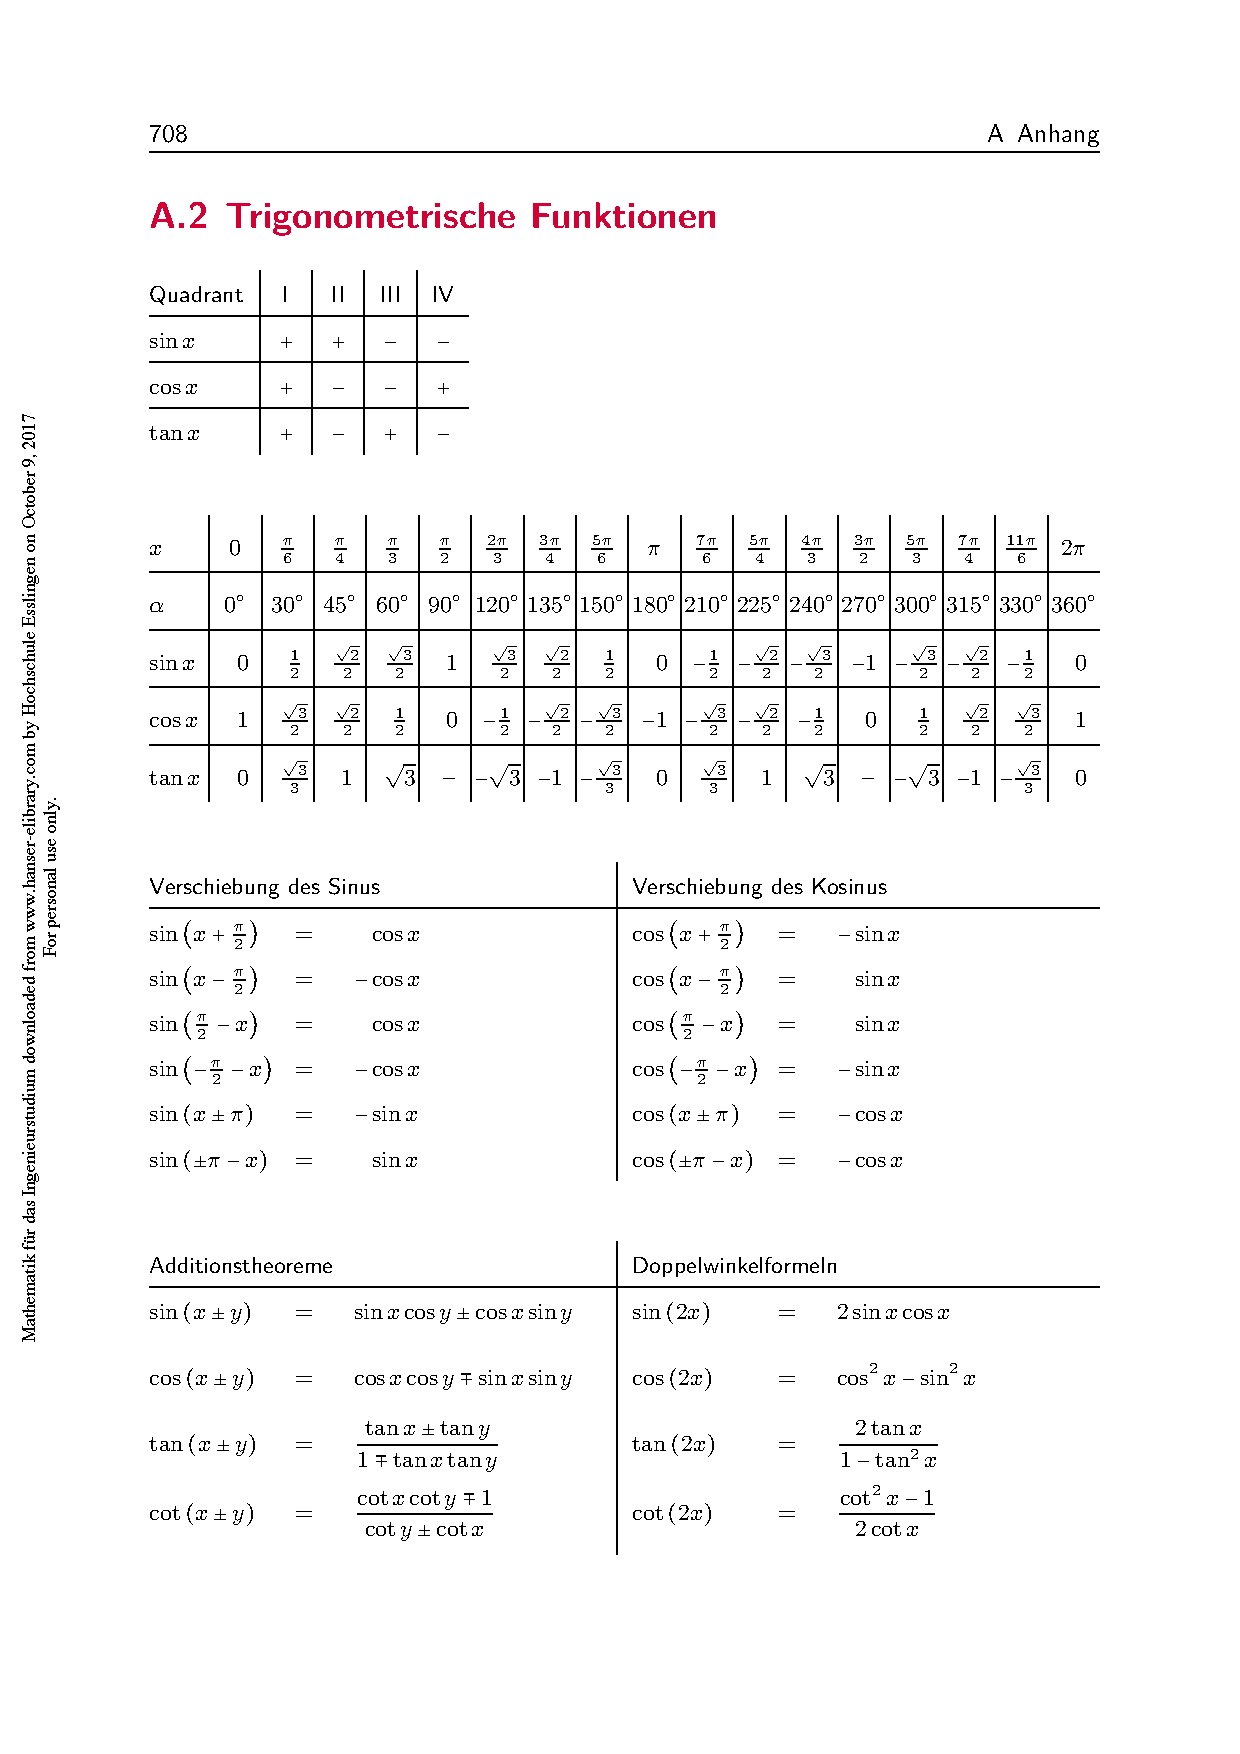
\includepdf[pages=-]{Cheatsheet.pdf}

\end{document}

%%% Local Variables:
%%% mode: latex
%%% TeX-master: t
%%% End:
